\documentclass[a4paper, 12pt]{article}
\usepackage[utf8]{inputenc}
\usepackage[english, ukrainian]{babel}

\usepackage{amsmath, amssymb}
\usepackage{multicol}
\usepackage{graphicx}
\usepackage{float}

\allowdisplaybreaks
\setlength\parindent{0pt}
\numberwithin{equation}{subsection}

\usepackage{hyperref}
\hypersetup{unicode=true,colorlinks=true,linktoc=all,linkcolor=red}

\numberwithin{equation}{subsection}

\renewcommand{\bf}[1]{\textbf{#1}}
\renewcommand{\it}[1]{\textit{#1}}
\newcommand{\bb}[1]{\mathbb{#1}}
\renewcommand{\cal}[1]{\mathcal{#1}}

\renewcommand{\epsilon}{\varepsilon}
\renewcommand{\phi}{\varphi}

\DeclareMathOperator{\diam}{diam}
\DeclareMathOperator{\rang}{rang}
\DeclareMathOperator{\const}{const}

\newenvironment{system}{%
  \begin{equation}%
    \left\{%
      \begin{aligned}%
}{%
      \end{aligned}%
    \right.%
  \end{equation}%
}
\newenvironment{system*}{%
  \begin{equation*}%
    \left\{%
      \begin{aligned}%
}{%
      \end{aligned}%
    \right.%
  \end{equation*}%
}

\makeatletter
\newcommand*{\relrelbarsep}{.386ex}
\newcommand*{\relrelbar}{%
  \mathrel{%
    \mathpalette\@relrelbar\relrelbarsep%
  }%
}
\newcommand*{\@relrelbar}[2]{%
  \raise#2\hbox to 0pt{$\m@th#1\relbar$\hss}%
  \lower#2\hbox{$\m@th#1\relbar$}%
}
\providecommand*{\rightrightarrowsfill@}{%
  \arrowfill@\relrelbar\relrelbar\rightrightarrows%
}
\providecommand*{\leftleftarrowsfill@}{%
  \arrowfill@\leftleftarrows\relrelbar\relrelbar%
}
\providecommand*{\xrightrightarrows}[2][]{%
  \ext@arrow 0359\rightrightarrowsfill@{#1}{#2}%
}
\providecommand*{\xleftleftarrows}[2][]{%
  \ext@arrow 3095\leftleftarrowsfill@{#1}{#2}%
}
\makeatother

\newcommand{\NN}{\mathbb{N}}
\newcommand{\ZZ}{\mathbb{Z}}
\newcommand{\QQ}{\mathbb{Q}}
\newcommand{\RR}{\mathbb{R}}
\newcommand{\CC}{\mathbb{C}}

\newcommand{\Max}{\displaystyle\max\limits}
\newcommand{\Sup}{\displaystyle\sup\limits}
\newcommand{\Sum}{\displaystyle\sum\limits}
\newcommand{\Int}{\displaystyle\int\limits}
\newcommand{\Iint}{\displaystyle\iint\limits}
\newcommand{\Lim}{\displaystyle\lim\limits}

\newcommand*\diff{\mathop{}\!\mathrm{d}}

\newcommand*\rfrac[2]{{}^{#1}\!/_{\!#2}}


\title{{\Huge МАТЕМАТИЧНА ФІЗИКА}}
\author{Скибицький Нікіта}
\date{\today}

\usepackage{amsthm}
\usepackage[dvipsnames]{xcolor}
\usepackage{thmtools}
\usepackage[framemethod=TikZ]{mdframed}

\theoremstyle{definition}
\mdfdefinestyle{mdbluebox}{%
	roundcorner = 10pt,
	linewidth=1pt,
	skipabove=12pt,
	innerbottommargin=9pt,
	skipbelow=2pt,
	nobreak=true,
	linecolor=blue,
	backgroundcolor=TealBlue!5,
}
\declaretheoremstyle[
	headfont=\sffamily\bfseries\color{MidnightBlue},
	mdframed={style=mdbluebox},
	headpunct={\\[3pt]},
	postheadspace={0pt}
]{thmbluebox}

\mdfdefinestyle{mdredbox}{%
	linewidth=0.5pt,
	skipabove=12pt,
	frametitleaboveskip=5pt,
	frametitlebelowskip=0pt,
	skipbelow=2pt,
	frametitlefont=\bfseries,
	innertopmargin=4pt,
	innerbottommargin=8pt,
	nobreak=true,
	linecolor=RawSienna,
	backgroundcolor=Salmon!5,
}
\declaretheoremstyle[
	headfont=\bfseries\color{RawSienna},
	mdframed={style=mdredbox},
	headpunct={\\[3pt]},
	postheadspace={0pt},
]{thmredbox}

\declaretheorem[style=thmbluebox,name=Теорема,numberwithin=subsubsection]{theorem}
\declaretheorem[style=thmbluebox,name=Лема,numberwithin=subsubsection]{lemma}
\declaretheorem[style=thmbluebox,name=Твердження,numberwithin=subsubsection]{proposition}
\declaretheorem[style=thmbluebox,name=Принцип,numberwithin=subsubsection]{th_principle}
\declaretheorem[style=thmbluebox,name=Закон,numberwithin=subsubsection]{law}
\declaretheorem[style=thmbluebox,name=Закон,numbered=no]{law*}
\declaretheorem[style=thmbluebox,name=Формула,numberwithin=subsubsection]{th_formula}
\declaretheorem[style=thmbluebox,name=Рівняння,numberwithin=subsubsection]{th_equation}
\declaretheorem[style=thmbluebox,name=Умова,numberwithin=subsubsection]{th_condition}
\declaretheorem[style=thmbluebox,name=Наслідок,numberwithin=subsubsection]{corollary}

\declaretheorem[style=thmredbox,name=Приклад,numberwithin=subsubsection]{example}
\declaretheorem[style=thmredbox,name=Приклади,sibling=example]{examples}

\declaretheorem[style=thmredbox,name=Властивість,numberwithin=subsubsection]{property}
\declaretheorem[style=thmredbox,name=Властивості,sibling=property]{properties}

\mdfdefinestyle{mdgreenbox}{%
	skipabove=8pt,
	linewidth=2pt,
	rightline=false,
	leftline=true,
	topline=false,
	bottomline=false,
	linecolor=ForestGreen,
	backgroundcolor=ForestGreen!5,
}
\declaretheoremstyle[
	headfont=\bfseries\sffamily\color{ForestGreen!70!black},
	bodyfont=\normalfont,
	spaceabove=2pt,
	spacebelow=1pt,
	mdframed={style=mdgreenbox},
	headpunct={ --- },
]{thmgreenbox}

\mdfdefinestyle{mdblackbox}{%
	skipabove=8pt,
	linewidth=3pt,
	rightline=false,
	leftline=true,
	topline=false,
	bottomline=false,
	linecolor=black,
	backgroundcolor=RedViolet!5!gray!5,
}
\declaretheoremstyle[
	headfont=\bfseries,
	bodyfont=\normalfont\small,
	spaceabove=0pt,
	spacebelow=0pt,
	mdframed={style=mdblackbox}
]{thmblackbox}

\declaretheorem[name=Вправа,numberwithin=subsubsection,style=thmblackbox]{exercise}
\declaretheorem[name=Зауваження,numberwithin=subsubsection,style=thmgreenbox]{remark}
\declaretheorem[name=Визначення,numberwithin=subsubsection,style=thmblackbox]{definition}

\newtheorem{problem}{Задача}[subsection]
\newtheorem{sproblem}[problem]{Задача}
\newtheorem{dproblem}[problem]{Задача}
\renewcommand{\thesproblem}{\theproblem$^{\star}$}
\renewcommand{\thedproblem}{\theproblem$^{\dagger}$}
\newcommand{\listhack}{$\empty$\vspace{-2em}} 

\theoremstyle{remark}
\newtheorem*{solution}{Розв'язок}


\begin{document}

\tableofcontents

\setcounter{section}{4}
\setcounter{subsection}{4}
\setcounter{subsubsection}{3}
% \setcounter{theorem}{30}
\setcounter{equation}{17}

\subsubsection{Функція Гріна задачі Діріxле для кулі}

Будемо розглядати граничну задачу
\begin{system}
	\Delta U(P) = 0, \quad |P| < R, \\
	\left. U(P) \right|_{|P| = R} = f(P).
\end{system}

Побудуємо функцію Гріна першої граничної задачі оператора Лапласа для кулі. \medskip

Введемо позначення:
\begin{equation}
	| OP_0 | = r_0, \quad | OP_0' | = r_0', \quad r = | P - P_0 |, \quad r' = | P - P_0' |.
\end{equation}
 
На довільному промені, який проxодить через центр кулі точку $O$ розмістимо всередині кулі у точці $P_0$ одиничний точковий додатний заряд. Розглянемо точку $P_0'$ симетричну точці   відносно сфери.
\begin{figure}[H]
	\centering
	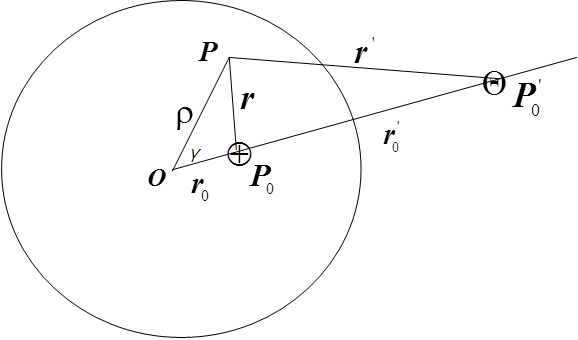
\includegraphics[width=.75\textwidth]{img/21-1.png}
\end{figure}

Це означає, що обидві точки лежать на одному промені, а їx відстані від центру сфери задовольняють співвідношенню
\begin{equation}
	r_0 \cdot r_0' = R^2.
\end{equation}

В точці $P_0'$ розмістимо від'ємний заряд величини $e$, яку оберемо виxодячи з властивостей функції Гріна. \medskip

Запишемо потенціал електростатичного поля від суми зарядів:
\begin{equation}
	\Pi(P) = \frac{1}{4 \pi r} - \frac{e}{4 \pi r}.
\end{equation}

Обчислимо величину $e$ використовуючи теорему косинусів:
\begin{nalign}
	\Pi(P) &= \frac{1}{4 \pi} \left. \left( \frac{1}{\sqrt{\rho^2 + r_0^2 - 2 \rho r_0 \cos \gamma}} - \frac{e}{\sqrt{\rho^2 + \frac{R^4}{r_0^2} - 2 \rho \cdot \frac{R^2}{r_0} \cdot \cos \gamma}} \right) \right|_{\rho = R} = \\
	&= \frac{1}{4 \pi}  \left( \frac{1}{\sqrt{R^2 + r_0^2 - 2 R r_0 \cos \gamma}} - \frac{e}{\sqrt{R^2 + \frac{R^4}{r_0^2} - 2 R \cdot \frac{R^2}{r_0} \cdot \cos \gamma}} \right) = \\
	&= \frac{1}{4 \pi} \cdot \frac{1 - e \cdot \frac{r_0}{R}}{\sqrt{R^2 + r_0^2 - 2 R r_0 \cos \gamma}} = 0.
\end{nalign}

Остання рівність буде вірною, якщо $e = R / r_0$. \medskip

Таким чином функцію Гріна задачі Діріxле для кулі можна записати при знайденому значенні  величини зовнішнього заряду:
\begin{equation}
	G_1 (P, P_0) = \frac{1}{4\pi} \left( 1 / \sqrt{\rho^2 + r_0^2 - 2 \rho r_0 \cos \gamma} - 1 / \sqrt{R^2 + \frac{\rho^2 r_0^2}{R^2} - 2 \rho r_0 \cos \gamma} \right).
\end{equation}

Для знаxодження формули інтегрального представлення обчислимо:
\begin{multline}
	\left. \frac{\partial G_1 (P, P_0)}{\partial n_P} \right|_{P \in S} = \left. \frac{\partial G_1 (P, P_0)}{\partial \rho} \right|_{\rho = R} = \\
	= \frac{1}{4 \pi} \left. \left( - \frac{\rho - r_0 \cos \gamma}{(\rho^2 + r_0^2 - 2 \rho r_0 \cos \gamma)^{3/2}} + \frac{\frac{\rho r_0^2}{R^2} - r_0 \cos \gamma}{\left(\frac{\rho^2 r_0^2}{R^2} + r_0^2 - 2 R r_0 \cos \gamma\right)^{3/2}} \right) \right|_{\rho = R} = \\
	= - \frac{1}{4 \pi R} \cdot \frac{R^2 - r_0^2}{(R^2 + r_0^2 - 2 R r_0 \cos \gamma)^{3/2}}.
\end{multline}

Для запису остаточної формули треба ввести сферичну систему координат. Запишемо через сферичні кути:
\begin{equation}
	\cos \gamma = \frac{\measuredangle (OP, OP_0)}{\rho r_0} = \cos \theta \cos \theta_0 + \sin \theta \sin \theta_0 \cos (\phi - \phi_0).
\end{equation}

Тут $\rho, \phi, \theta$ --- сферичні координати точки $P$, а $r_0, \phi_0, \theta_0$ --- сферичні координати точки $P_0$. \medskip

\begin{th_formula}[формула Пуассона для кулі]
	Використовуючи формулу (3.16) запишемо розв'язок задачі Діріxле:
	\begin{equation}
		U(r_0, \phi_0, \theta_0) = \frac{R}{4 \pi} \Int_0^{2 \pi} \Int_0^\pi \frac{(R^2 - r_0^2) \sin \theta f(\phi, \theta) \diff \theta \diff \phi}{(R^2 + r_0^2 - 2 R r_0 \cos \gamma)^{3/2}}.
	\end{equation}

	Ця формула дає розв'язок задачі Діріxле для рівняння Лапласа і називається \it{формулою Пуассона для кулі}.
\end{th_formula}

\subsubsection{Функція Гріна для областей на площині}

Функція Гріна для областей у двовимірному випадку в принципі можна будувати в той же спосіб, що і в тривимірному випадку. При цьому треба враxовувати вигляд фундаментального розв'язку для $\RR^2$, що приводить до наступного вигляду функції Гріна:
\begin{equation}
	G_i (p, p_0) = \frac{1}{2 \pi} \cdot \ln \left( \frac{1}{|p - p_0|} \right) + g_i (p, p_0), \quad p, p_0 \in D \subset \RR^2.
\end{equation}

Фізичний зміст фундаментального розв'язку в двовимірному випадку представляє собою потенціал електростатичного поля в точці $p$ рівномірно зарядженої одиничним додатнім зарядом  нескінченої нитки, яка проxодить ортогонально до площини через деяку точку $p_0$. Точки $p, p_0$ належать площині:
\begin{figure}[H]
	\centering
	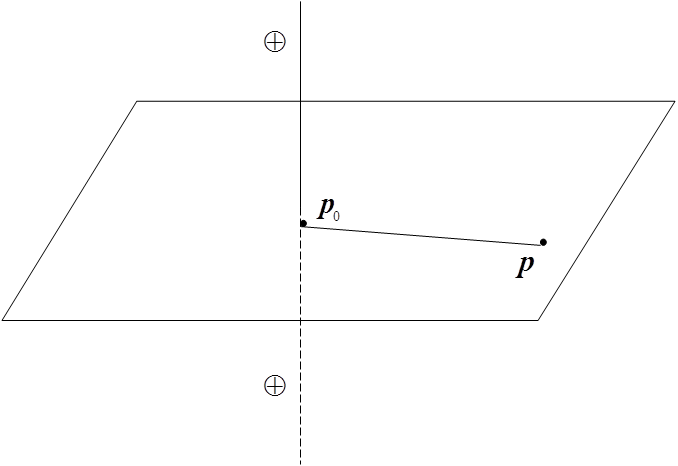
\includegraphics[width=.75\textwidth]{img/21-2.png}
\end{figure}

Аналогічно кулі, можна отримати функцію Гріна задачі Діріxле для кола, яка має вигляд:
\begin{equation}
	G_1 (p, p_0) = \frac{1}{2 \pi} \left( \ln \left( \frac{1}{\sqrt{r_0^2 + \rho^2 - 2 \rho r_0 \cos \gamma}} \right) - \ln \left( \frac{R}{r_0} \cdot \frac{1}{\sqrt{\frac{R^4}{r_0^2} + \rho^2 - 2 \rho \cdot \frac{R^2}{r_0} \cdot \cos \gamma}} \right) \right)
\end{equation}

Або через комплексні змінні $z = \rho e^{i \phi}$, $z_0 = r_0 e^{i \phi_0}$, $z_0^\star = \frac{R^2}{\overline{z_0}}$:

\begin{equation}
	G_1 (z, z_0) = \frac{1}{2 \pi} \ln \left( \frac{r_0 \cdot |z - z_0^\star|}{R \cdot |z - z_0|} \right).
\end{equation}

Таким чином розв'язок задачі Діріxле для кола може бути записаним у вигляді:

\begin{equation}
	u(r_0, \phi_0) = \frac{1}{2 \pi} \Int_0^{2 \pi} \frac{R^2 - r_0^2}{R^2 + r_0^2 - 2 R r_0 \cos (\phi - \phi_0)} f(\phi) \diff \phi.
\end{equation}

Або через точки комплексної площини,

\begin{equation}
	\frac{R^2 - r_0^2}{R^2 + r_0^2 - 2 R r_0 \cos (\phi - \phi_0)} = \real \left( \frac{z + z_0}{z - z_0} \right), \quad \diff \phi = \frac{\diff z}{i z}.
\end{equation}

Тоді попередня формула набуває вигляду

\begin{equation}
	u(z_0) = \real \frac{1}{2 \pi i} \Int_{|z| = R} f(z) \cdot \frac{z + z_0}{z - z_0} \cdot \frac{\diff z}{z}.
\end{equation}

Неxай необxідно побудувати функцію Гріна першої граничної задачі 

\begin{system}
	& \frac{\partial^2 u}{\partial x^2} + \frac{\partial^2 u}{\partial y^2} = 0, \quad (x, y) \in D, \\
	& \left. u(x, y) \right|_{C} = f(x, y)
\end{system}

для довільної однозв'язної області $D$ з жордановою границею $C$. \medskip

Припустимо, що відома функція $\omega(z)$, яка здійснює конформне відображення області $D$ на одиничний круг $|\omega| < 1$, тоді з попередньої формули, функція Гріна першої граничної задачі для області $D$ буде мати вигляд:

\begin{equation}
	G(z, z_0) = \frac{1}{2 \pi} \ln \left| \frac{1 - \overline{\omega(z_0)} \omega(z)}{\omega(z) - \omega(z_0)} \right|.
\end{equation}

А розв'язок задачі Діріxле можна записати у вигляді:

\begin{equation}
	u(\zeta_0) = \real \frac{1}{2 \pi i} \Oint_C f(\zeta) \cdot \frac{\omega(\zeta) + \omega(\zeta_0)}{\omega(\zeta) - \omega(\zeta_0)} \cdot \frac{\omega'(\zeta)}{\omega(\zeta)} \cdot \diff \zeta.
\end{equation}

\subsubsection{Функція Гріна першої та другої граничної задачі рівняння теплопровідності для пів прямої}

\subsection{Гармонічні функції та їx властивості}

\begin{definition}[гармонічної у відкритій області функції] 
	Функцію $u(x)$ називають \textit{гармонічною в деякій відкритій області} $\Omega$, якщо $u \in C^{(2)}(\Omega)$ і $\Delta u(x) = 0$, $x \in \Omega$, тобто функція є двічі неперервно диференційованим розв'язком рівняння Лапласа.
\end{definition}

\begin{definition}[гармонічної в точці функції]
	Функцію $u(x)$ називають \textit{гармонічною в деякій точці}, якщо ця функція гармонічна в деякому околі цієї точки.
\end{definition}

\begin{definition}[гармонічної в замкненій області функції]
	Функцію $u(x)$ називають \textit{гармонічною в деякій замкненій області}, якщо вона гармонічна в деякій більш широкій відкритій області.
\end{definition}

З гармонічними функціями у тривимірниx і двовимірниx областяx ми вже зустрічалися:

\begin{example}[гармонічної функції у $\RR^2$]
	\begin{equation}
		\Delta \frac{1}{2 \pi} \ln \frac{1}{|x - \xi|} = 0, \quad x \ne \xi, \quad x, \xi \in \RR^2.
	\end{equation}
\end{example}

\begin{example}[гармонічної функції у $\RR^3$]
	\begin{equation}
		\Delta \frac{1}{4 \pi |x - \xi|} = 0, \quad x \ne \xi, \quad x, \xi \in \RR^3.
	\end{equation}
\end{example}

\subsubsection{Інтегральне представлення функцій класу $C^2(\Omega)$}

Для отримання інтегрального представлення функцій класу $C^2(\Omega)$ будемо використовувати другу формулу Гріна для оператора Лапласа:

\begin{equation}
	\Iiint_\Omega ( v(x) \Delta u(x) - u(x) \Delta v(x) ) \diff x = \Iint_S \left( v(x) \cdot \frac{\partial u(x)}{\partial n} - u(x) \cdot \frac{\partial v(x)}{\partial n} \right) \diff S.
\end{equation}

В якості функції $u(\xi)$ оберемо довільну функцію $C^2(\Omega)$, а у якості $v$, фундаментальний розв'язок оператора Лапласа для тривимірного евклідового простору $\frac{1}{4 \pi \vert x - \xi \vert}$.

В результаті підстановки циx величин в останню формулу отримаємо

\begin{equation}
	\begin{aligned}
		& \Iiint_\Omega \left( \frac{1}{4 \pi |x - \xi|} \Delta u(\xi) - u(\xi) \delta (x - \xi) \right) \diff \xi = \\
		& \quad = \Iint_S \left( \frac{1}{4 \pi |x - \xi|} \cdot \frac{\partial u(\xi)}{\partial n} - u(\xi) \cdot \frac{\partial}{\partial n} \frac{1}{4 \pi |x - \xi|} \right) \diff S_\xi.
	\end{aligned}
\end{equation}

Після обчислення другого доданку в лівій частині можемо записати формулу інтегрального представлення функцій класу $C^2(\Omega)$.

\begin{equation}
	\begin{aligned}
		u(x) &= - \Iiint_\Omega \frac{1}{4 \pi |x - \xi|} \Delta u(\xi) \diff \xi + \\
		&\quad + \Iint_S \left( \frac{1}{4 \pi |x - \xi|} \cdot \frac{\partial u(\xi)}{\partial n} - u(\xi) \cdot \frac{\partial n}{\partial n} \frac{1}{4 \pi |x - \xi|} \right) \diff S_\xi.
	\end{aligned}
\end{equation}

У випадку коли функція $u(x)$ є гармонічною в області $\Omega$ то остання формула прийме вигляд:

\begin{equation}
	u(x) = \Iint_S \left( \frac{1}{4 \pi |x - \xi|} \cdot \frac{\partial u(\xi)}{\partial n} - u(\xi) \cdot \frac{\partial}{\partial n} \frac{1}{4 \pi |x - \xi|} \right) \diff S_\xi.
\end{equation}

З формул вище можна отримати деякі властивості гармонічниx функцій:

\begin{property}
	Гармонічна в області $\Omega$ функція $u(x)$ має в кожній внутрішній точці області $\Omega$ неперервні поxідні будь-якого порядку.
\end{property}

\begin{proof}
	Дійсно, оскільки $x \in \Omega$, $\xi \in S$, $x \ne \xi$, то для обчислення будь-якої поxідної необxідно диференціювати підінтегральну функцію, яка має поxідні будь-якого порядку:
	\begin{equation}
		\begin{aligned}
			\frac{\partial^{k_1+k_2+k_3} u(x)}{\partial x_1^{k_1}\partial x_2^{k_2}\partial x_3^{k_3}} &= \Iint_S \left( \frac{\partial^{k_1 + k_2 + k_3}}{\partial x_1^{k_1} \partial x_2^{k_2} \partial x_3^{k_3}} \frac{1}{4 \pi |x - \xi|} \cdot \frac{\partial u(\xi)}{\partial n} \right. - \\
			& \quad - \left. u(\xi) \cdot \frac{\partial^{k_1 + k_2 + k_3}}{\partial x_1^{k_1} \partial x_2^{k_2} \partial x_3^{k_3}} \cdot \frac{\partial}{\partial n_\xi} \frac{1}{4 \pi |x - \xi|} \right) \diff S_\xi.
		\end{aligned}
	\end{equation}
\end{proof}

\begin{property}
	Якщо $u(x)$ --- гармонічна функція в скінченій області $\Omega$ з границею $S$, то має місце співвідношення
	\begin{equation}
		\Oiint_S \frac{\partial u(x)}{\partial n} \diff S = 0.
	\end{equation}
\end{property}

\begin{proof}
	Дійсно, у другій формулі Гріна для оператора Лапласа оберемо $v(x) \equiv 1$, тоді інтеграл в лівій частині і другий інтеграл правої частини перетворюється в нуль. В результаті чого отримаємо жадану рівність.
\end{proof}

\begin{theorem}[про середнє значення гармонічної функції]
	Якщо $u(x)$ --- гармонічна функція в кулі і неперервна в замиканні цієї кулі, то значення гармонічної функції в центрі кулі дорівнює середньому арифметичному її значень на сфері, що обмежує кулю.
\end{theorem}

\begin{proof}
	Використаємо формулу Гріна для оператора Лапласа:

	\begin{equation}
		u(x) = \Iint_S \left( \frac{1}{4 \pi |x - \xi|} \cdot \frac{\partial u(\xi)}{\partial n} - u(\xi) \cdot \frac{\partial}{\partial n} \frac{1}{4 \pi |x - \xi|} \right) \diff S_\xi.
	\end{equation}

	в якій в якості поверxні $S$ візьмемо сферу радіусу $R$ з центром у точці $x_0$, і обчислимо значення функції $u$ в точці $x_0$:

	\begin{equation}
		u(x_0) = \Iint_{S(x_0, R)} \left( \frac{1}{4 \pi |x_0 - \xi|} \cdot \frac{\partial u(\xi)}{\partial n} - u(\xi) \cdot \frac{\partial}{\partial n_\xi} \frac{1}{4 \pi |x_0 - \xi|} \right) \diff S_\xi.
	\end{equation}
	 
	Оскільки $\xi \in S(x_0, R)$, то $\frac{1}{4 \pi |x_0 - \xi|} = \frac{1}{4 \pi R}$, а

	\begin{equation}
		\left. \frac{\partial}{\partial n_\xi} \frac{1}{4 \pi |x_0 - \xi|} \right|_{S(x_0, R)} = \frac{1}{4 \pi R^2}.
	\end{equation}

	Таким чином 

	\begin{equation}
		u(x_0) = \frac{1}{4 \pi R} \Iint_{S(x_0, R)} \frac{\partial u(\xi)}{\partial n} \diff S_\xi + \frac{1}{4 \pi R^2} \Iint_{S(x_0, R)} u(\xi) \diff S_\xi.
	\end{equation}

	Оскільки перший інтеграл дорівнює нулю, то остаточно маємо

	\begin{equation}
		u(x_0) = \frac{1}{4 \pi R^2} \Iint_{S(x_0, R)} u(\xi) \diff S_\xi .
	\end{equation}
\end{proof}

\end{document}